\documentclass[conference]{IEEEtran}
%\IEEEoverridecommandlockouts
%The preceding line is only needed to identify funding in the first footnote. If that is unneeded, please comment it out.
\usepackage{cite}
\usepackage{amsmath,amssymb,amsfonts}
\usepackage{algorithmic}
\usepackage{graphicx}
\usepackage{textcomp}
\usepackage{xcolor}
\def\BibTeX{{\rm B\kern-.05em{\sc i\kern-.025em b}\kern-.08em
    T\kern-.1667em\lower.7ex\hbox{E}\kern-.125emX}}

\renewcommand{\baselinestretch}{1.08}

\begin{document}

\title{A LSTM-Based Syncretic Positioning Model Working Under Any Environment in SaaS \\
%{\footnotesize \textsuperscript{*}Note: Sub-titles are not captured in Xplore and
%should not be used}
%\thanks{Identify applicable funding agency here. If none, delete this.}
}

\author{\IEEEauthorblockN{1\textsuperscript{st} Zhen-Qiang Sun}
\IEEEauthorblockA{\textit{School of Computer and Electronic Information / School of Artificial Intelligence} \\
\textit{Nanjing Normal University}\\
Nanjing, China \\
enderman19980125@outlook.com}
%\and
%\IEEEauthorblockN{2\textsuperscript{nd} Given Name Surname}
%\IEEEauthorblockA{\textit{dept. name of organization (of Aff.)} \\
%\textit{name of organization (of Aff.)}\\
%City, Country \\
%email address}
%\and
%\IEEEauthorblockN{3\textsuperscript{rd} Given Name Surname}
%\IEEEauthorblockA{\textit{dept. name of organization (of Aff.)} \\
%\textit{name of organization (of Aff.)}\\
%City, Country \\
%email address}
%\and
%\IEEEauthorblockN{4\textsuperscript{th} Given Name Surname}
%\IEEEauthorblockA{\textit{dept. name of organization (of Aff.)} \\
%\textit{name of organization (of Aff.)}\\
%City, Country \\
%email address}
%\and
%\IEEEauthorblockN{5\textsuperscript{th} Given Name Surname}
%\IEEEauthorblockA{\textit{dept. name of organization (of Aff.)} \\
%\textit{name of organization (of Aff.)}\\
%City, Country \\
%email address}
%\and
%\IEEEauthorblockN{6\textsuperscript{th} Given Name Surname}
%\IEEEauthorblockA{\textit{dept. name of organization (of Aff.)} \\
%\textit{name of organization (of Aff.)}\\
%City, Country \\
%email address}
}

\maketitle

\begin{abstract}
Positioning technology is particularly important in today's highly developed information technology. GPS positioning, which started early, can meet the positioning needs in most scenarios, but GPS has poor positioning accuracy in indoor environments. Therefore, positioning algorithms such as Wi-Fi fingerprint positioning and PDR positioning have been proposed. When the mobile device is in a complex scene, the positioning model should be dynamically switched according to different scenes. This paper proposes the SPAE model, which is an ensemble algorithm. Three common positioning modules are integrated in the SPAE model, namely GPS positioning, Wi-Fi fingerprint positioning, and PDR positioning. The SPAE model uses the LSTM network to dynamically adjust the weight parameters of the three positioning modules to adapt to the positioning model selection problem in complex scenes. Experiments show that the SPAE model can dynamically adjust the parameters of the positioning module according to the scene, and achieve high-precision positioning in complex scenes.
\end{abstract}

\begin{IEEEkeywords}
positioning system, indoor localization, Wi-Fi fingerprinting, long short-term memory (LSTM), system deployment,  software-as-a-service (SaaS)
\end{IEEEkeywords}

\section{Introduction}
In today's society, positioning technology has penetrated into all aspects of our daily lives. Almost all smart phones have built-in positioning modules. It is undeniable that positioning technology has brought great convenience to people's daily travel. Thanks to the location information of the smartphone, the application can provide users with relevant services in the current area. For example, a taxi-hailing application can search for available vehicles and allocate orders in the area near the user, a social application can recommend nearby friends for the user to chat, and a game application can match players near the user to reduce network latency.

In recent years, the research and application of many emerging technologies are inseparable from the support of positioning technology, such as the Internet of Things technology and unmanned driving technology. Some examples are shown in Fig. \ref{fig:applications}. It can be said that positioning technology has changed our way of life, some previously impossible tasks have become reality, and the social living environment continues to provide a broad stage for positioning technology.

\begin{figure}[t]
	\centering
	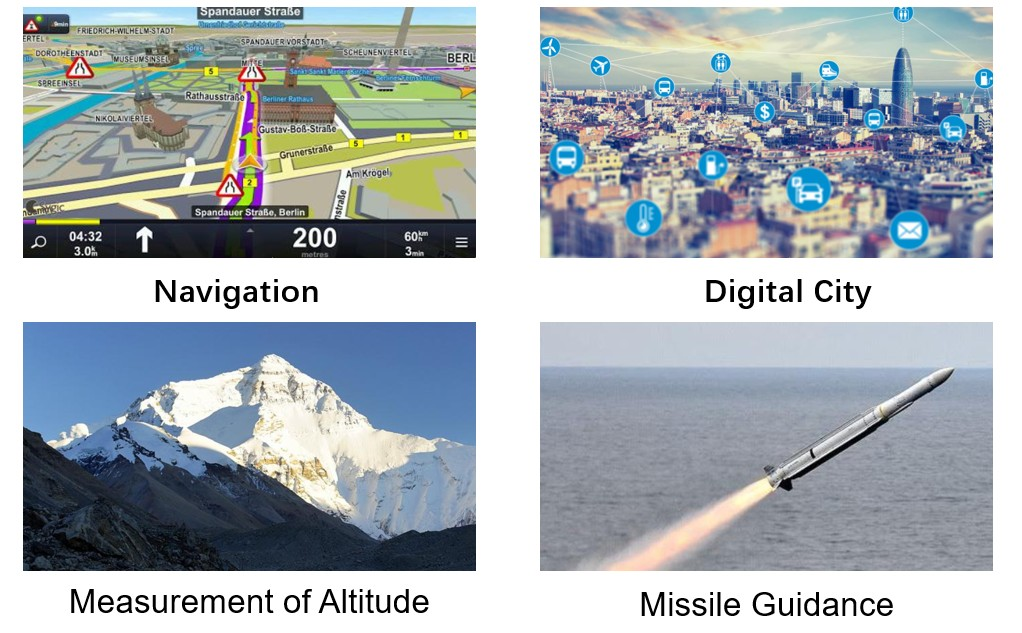
\includegraphics[scale=0.4]{./figures/applications.jpg}
	\caption{the Applications of Positioning Technology}
	\label{fig:applications}
\end{figure}

SaaS (Software-as-a-Service) is a completely innovative software application model that has emerged in the 21st century with the development of Internet technology and the maturity of application software. In the traditional mode, vendors use licenses to deploy software products to multiple client terminals within the enterprise for delivery. SaaS defines a new delivery method, and also makes software return to the essence of service. The essence of enterprise deployment of informatization software is for its own operation and management services. The appearance of software is the informatization of business processes, and the essence is still the first service model. SaaS has changed the way of providing traditional software services and reduced the need for local deployment. A large amount of early-stage investment, further highlighting the service attributes of informatization software, or becoming the mainstream delivery mode of the informatization software market in the future.

Developers have always hoped to distribute the positioning module as a service to customers, which can not only effectively reduce operating costs, but also use big data to analyze historical records to further improve the accuracy of positioning technology. All of them try to provide SaaS (software as a service) by giving out an SDK for the developers to program various applications on top of their location service to run in their smartphones.\cite{intro-saas}

At the same time, positioning technology is also an important part of digital smart cities. The vigorous development of the Internet of Things and wireless sensor technology has promoted tremendous changes in information technology and industry. Smart cities have transformed from the original concept to the application of technology that is closely related to people's lives. As one of the indispensable cornerstones of urban infrastructure construction, positioning technology is widely used in the fields of transportation, medical treatment, and home furnishing.

With the development of wireless communication technology and the penetration of smart devices in daily life, indoor positioning technology has also attracted more and more attention, and people's demand for high-precision positioning has become increasingly strong. \cite{intro-cloud} Indoor positioning technology has corresponding service requirements in large shopping malls, museums, office buildings, underground parking rooms, logistics warehouses, etc., such as recommending nearby businesses to users and preferential activities to drive consumption, and museums provide corresponding exhibits In the smart medical system, indoor positioning can be used to realize the health care of patients, electronic medical guidance, and emergency rescue. In the indoor environment, the satellite signal is relatively weak, and the Beidou satellite navigation system cannot meet the positioning accuracy requirements.

The difficulty of current positioning technology lies in precise positioning in an indoor environment. Part of the existing indoor positioning technology is based on wireless signal propagation characteristics such as Wi-Fi and Bluetooth. This type of positioning solution can achieve higher accuracy, and usually requires the deployment of signal transmitting beacons or receivers, etc., which are suitable for places where indoor facilities are relatively stable; partly, inertial sensor data is used to analyze user walking characteristics to achieve positioning purposes. This kind of method has low cost and strong versatility, but the accuracy is not high. Due to the complex and changeable indoor environment, there is no high-performance positioning technology that can well meet the current indoor positioning needs.

The rest of this article is structured as follows: in Section II, we introduced two classifications of positioning technology-outdoor positioning and indoor positioning. Among them, we focused on indoor positioning related research. Indoor positioning is also the current overall positioning technology research Difficulties and hot spots. In Section III, we elaborated on the fusion positioning algorithm proposed in this article. In Section IV, we elaborated on the simulation experiment conducted in the virtual environment, and conducted an in-depth analysis and analysis of the experimental results. Finally, Section V concludes the study.

\section{Related Work}
According to different environments, positioning technologies can be divided into two categories, namely outdoor positioning and indoor positioning. Outdoor positioning refers to the positioning of the device when it is in an open environment, such as on the street, in the field, in the woods, etc. Indoor positioning refers to the positioning of equipment when it is in a closed environment, such as in a room, banquet hall, underground parking lot, etc. However, there is no strict boundary between outdoor positioning and indoor positioning, but when the device is in a different environment, the positioning model and correction algorithm used will be different. \cite{env-urban}. The categories of positioning technology are shown in Fig. \ref{fig:category}.

\begin{figure}[t]
	\centering
	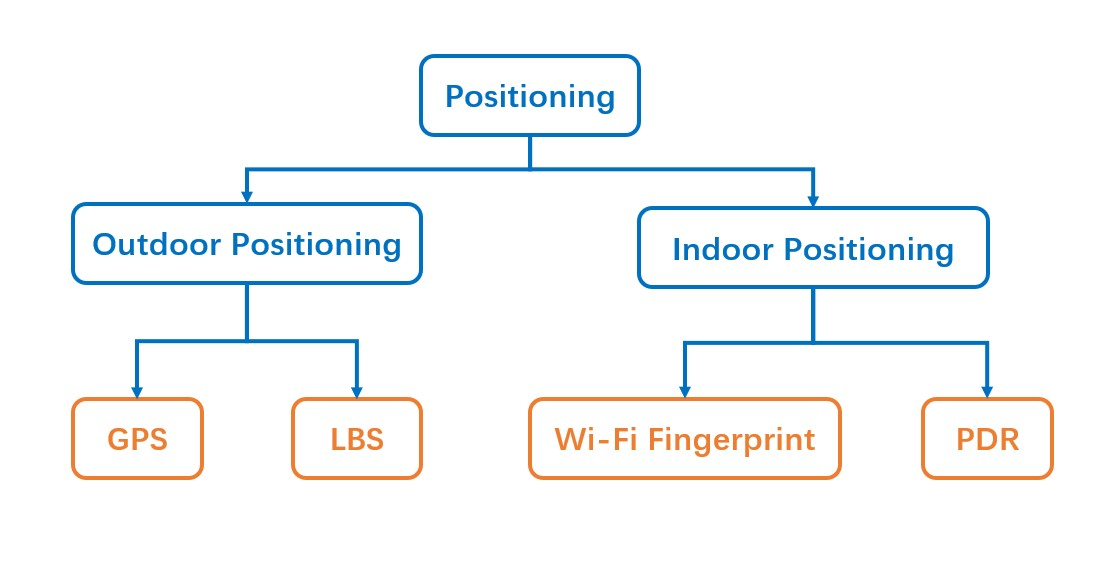
\includegraphics[scale=0.4]{./figures/category.jpg}
	\caption{the Categories of Positioning Technology}
	\label{fig:category}
\end{figure}

Traditional positioning modes include satellite-based positioning and base station-based positioning, which are also two positioning modes that are currently mature and widely used. In recent years, with the rapid development of deep learning, deep neural networks are playing an unprecedented and huge role in all walks of life, and have achieved many excellent research results and technical applications. \cite{env-cv} is no exception in the field of positioning. Neural networks, especially cyclic neural networks, play a huge role in trajectory prediction and position correction, and they are also one of the current hot issues in academic research. \cite{gps-1}
Outdoor positioning. The current outdoor positioning technology is very mature, mainly divided into GNSS positioning and LBS positioning.

LBS positioning is base station positioning, which obtains the location information of mobile terminal users through the networks of telecommunications mobile operators (such as GSM networks, GPRS, etc.). The positioning principle is that after the user turns on the positioning service, it will search for all nearby base stations. Of course, the distance between you and each base station is different, and the signal strength received at the distance is also different. When the received base station is greater than or equal to 3, the approximate position can be obtained according to the three-point positioning. \cite{indoor-review} Due to the instability of the signal, the positioning accuracy is about several hundred meters. However, since the base station positioning value receives the signal from the base station, the power consumption is relatively small. Of course, scanning the base station is a waste of electricity.

GNSS positioning is the global navigation satellite system, which includes GPS in the United States, Glonass in Russia, Galileo in Europe, Beidou satellite navigation system in China and related auxiliary systems. Many positioning systems including the Global Positioning System (GPS) have already existed in the world. The \cite{gps-2} navigation system is extremely important to the country’s economic development and safety. Therefore, Chinese researchers have put a lot of effort into building a satellite navigation system. In 2020, the deployment of all constellations of the Beidou navigation system has finally been completed, and it will provide global users with all-weather, all-weather, high-precision positioning, navigation and timing services.

The advantages of GPS positioning are 1) High positioning accuracy, ordinary civilian level positioning accuracy can reach 5-10m, military level positioning accuracy can reach a few centimeters; 2) wide range, almost anywhere on the earth can receive satellite signals , So there are almost no areas that cannot be located; but the disadvantages are 1) High investment cost. The cost of developing a satellite positioning system includes system research and development costs, satellite research and development costs, and maintenance and operation costs. At present, the basic satellite positioning systems in the world are It is developed and constructed by a large country with the strength of the whole country; 2) The device has high power consumption, and the satellite positioning service is provided by the built-in GPS module of the device, and the GPS module is a very power-consuming module in the device, which will occupy a lot of system resources; 3) Affected by weather and location, the GPS receiving antenna of the device must be outdoors and can see a large area to fill in the blank, otherwise the signal strength will be seriously affected, leading to positioning deviation and delay.

The advantages of LBS positioning are 1) fast positioning speed, and the positioning function is not restricted by factors such as weather and tall buildings; 2) low power consumption of the device, as long as the base station collects data, it does not consume the power of the mobile phone; the disadvantage is 1) low positioning accuracy. The urban area is only 20-200 meters, and the suburban areas are only 1000-2000 meters; 2) Depending on the base station, the positioning condition must be at the location where the base station signal is available, the mobile phone is in the sim card registration state, and the signals from at least 3 base stations must be received.

By analyzing and comparing the advantages and disadvantages of GPS positioning and LBS positioning, we can see that the positioning accuracy of GPS in an outdoor environment is very high, while in an indoor environment, the positioning accuracy is very low due to weak satellite signals received. The positioning accuracy of the LBS positioning itself is very low, which leads to the generally low positioning accuracy in the indoor environment. But this is precisely the opposite of what people want. Because the outdoor environment is often relatively compact, if you want to build an indoor navigation application, the deviation of tens of meters is unacceptable. \cite{indoor-precision} Therefore, how to effectively improve the accuracy of indoor positioning has always been an urgent problem to be solved in academia, and it is also one of the current research hotspots.

There are many types of existing indoor positioning technologies, and their principles can be divided into five categories: wireless signal convergence positioning, database matching positioning, inertial sensor-based track calculation positioning (PDR), visual positioning and multi-sensor combined positioning. Wireless signal convergence positioning obtains the current position of the positioning target by calculating the distance from each signal sending end to the receiving end. The representative ones are the trilateral positioning method \cite{indoor-3edges}, and the distance measurement method based on the time of arrival (ToA)\cite {indoor-toa} etc. The trilateral positioning method first obtains three candidate points near the positioning target. In an ideal state, the target point will be at the intersection of three circles with the candidate point as the center and radius as the distance. However, there is a multipath effect during wireless signal propagation, and it is easily affected by indoor objects on the way to produce reflection, diffraction or refraction, causing the collected signal to be greatly affected by noise. The three circles do not intersect at one point, and further screening and processing are required to obtain the final positioning. coordinate.

Based on the uniqueness of the signal's characteristics in each part of the room, the database matching positioning method regards the signal characteristics as fingerprints, and the mobile terminal collects location information and sends it to the server. A specific algorithm is used to match the location closest to the signal feature of the positioning target in the database. coordinate. \cite{indoor-fp1}\cite{indoor-fp1} proposes a geomagnetic fingerprint indoor positioning system based on learning sequence, but the geomagnetic signal is greatly affected by metal, and magnetic nails need to be deployed on the indoor ground. The use scenarios are limited. Parking lots or warehouses are used more often.

In recent years, the popularization of smart phones has continued to expand. Mobile terminals generally integrate inertial sensors (IMUs) that measure acceleration, deflection angular velocity, and heading angle. From these data, the step length and direction of pedestrians can be calculated. IMU is used in pedestrian track estimation It is widely used.\cite{indoor-imu1} Integrating the data collected by mobile terminal inertial sensors, Wi-Fi and iBeacon, proposes a Wi-Fi and PDR fusion positioning and navigation system, and uses the OS-ELM model to quickly extract Wi-Fi fingerprint information, Establish a fingerprint database to determine the initial position of the pedestrian and correct the PDR drift problem.\cite{indoor-imu2} also uses the WiFi signal to obtain the initial position of the pedestrian, but the difference is that they use the signal attenuation algorithm to calculate the distance from each signal source to the movement The distance of the receiving end can be obtained to obtain the starting point, improve the real-time positioning, and then use the Kalman filter to remove the noise in the inertial sensor data, and mark the landmark to solve the PDR drift problem.

The above are relatively traditional indoor positioning methods, and there is currently no mature, stable and widely used high-precision indoor positioning technology. \cite{indoor-no} With the emergence of computer computing power, storage capacity, and various excellent algorithms, artificial intelligence is developing in full swing, and researchers can integrate traditional positioning technology with artificial intelligence technology.

\begin{figure}[h]
	\centering
	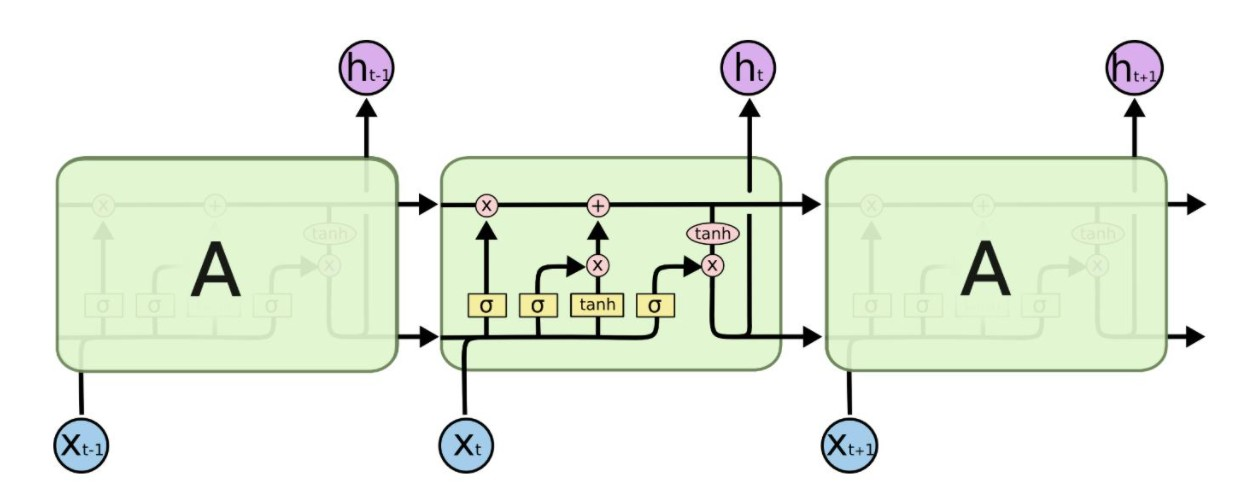
\includegraphics[scale=0.3]{./figures/lstm.jpg}
	\caption{the Structure of a LSTM Network}
	\label{fig:lstm}
\end{figure}

Especially with the large-scale application of LSTM \ref{fig:lstm} and Attention mechanism \cite{attention}, deep learning is playing an extraordinary role in the field of indoor positioning. A common LSTM single cell structure is shown in Fig. \ref{fig:lstm}. Some researchers began to apply the deep learning neural network framework to indoor positioning. \cite{indoor-lstm} proposes an indoor Wi-Fi fingerprint location algorithm based on LSTM. LSTM is generally suitable for classification, processing and prediction based on time series data. \cite{indoor-deep1} proposes an indoor fingerprint recognition system based on deep learning, which combines RSSI and magnetic field to form fingerprints with more complete information, and uses deep learning to extract fingerprints' intrinsic characteristics, which is helpful to improve positioning accuracy. \cite{indoor-deep2} proposed an indoor location algorithm (DL-IMPS) based on multi-sensor fingerprints and deep learning, and used statistical models and ray tracing methods to construct large sample data for weight training.

\section{SPAE Algorithm}
At present, the existing algorithms can basically only adapt to a single simple scene, but can't do anything for complex and changeable composite scenes. For example, when the device moves from the basement to the street, the corresponding positioning algorithm should be switched from a certain indoor positioning algorithm to GPS positioning, and vice versa. In this regard, we proposed the SPAE algorithm (a Syncretic Positioning model working under Any Environment), which helps to realize intelligent switching between composite scenes. In the first part, we elaborated on the various positioning modules of the SPAE algorithm, and in the second part, we elaborated on the working process of the SPAE algorithm and the processing of time streaming data by the LSTM network.

\subsection{Modules of SPAE}
The SPAE algorithm is essentially an ensemble algorithm, which is composed of three different basic positioning algorithm modules. These basic positioning algorithm modules include GPS positioning module, Wi-Fi fingerprint positioning module, and PDR positioning module. These three positioning algorithms are currently mature positioning algorithms and have been applied on a large scale on mobile devices. Below, we respectively introduce the working principles of these three modules.

\subsubsection{GPS Positioning Module}
GPS is a well-known satellite positioning system. In a narrow sense, it refers to the satellite positioning system established by the United States, and in a broad sense, it refers to any satellite-based global positioning system, such as China's Beidou, Russia's Glonass, and Europe's Galileo. This article adopts a broad definition. GPS positioning is currently the most accurate and widely used positioning and navigation technology, and it will become one of the standard configurations of every mobile device in the future. Today's mid-to-high end can only be mobile phones, and quite a few are already equipped with GPS hardware.

Take the GPS of the United States as an example, the GPS space part is mainly composed of 24 GPS satellites, of which 21 are working satellites and 3 are spare satellites. The 24 satellites operate on 6 orbital planes, and the operation period is 12 hours. It is guaranteed that more than 4 satellites can be observed at any time and at any location with an elevation angle of 15 degrees or more. The GPS control part is composed of 1 main control station, 5 detection stations and 3 injection stations. The GPS user equipment part includes GPS receivers and related equipment. The GPS receiver is mainly composed of GPS chips.

Below we explain the positioning principle of GPS. Each of the GPS satellites operating in space constantly broadcasts its current position coordinate information to the world through satellite signals. Any GPS receiver can easily receive this information through the antenna, and can read this information, which is actually one of the core functions of every GPS chip. This is the source of these location information.

Since every GPS satellite is working tirelessly to broadcast its position, when sending the position information, it will also attach the time stamp when the data packet is sent. After the GPS receiver receives the data packet, it subtracts the time on the timestamp from the current time, which is the time it takes for the data packet to be transmitted in the air. Knowing the transmission time of the data packet in the air, then multiplying it by its transmission speed is the distance of the data packet transmission in the air, that is, the distance between the satellite and the GPS receiver.

According to the knowledge of solid geometry, in a three-dimensional space, three pairs of coordinate points can uniquely determine a point (in fact, there may be two, but we can discard one through logical judgment). This type of positioning is called single-point positioning, or absolute positioning. The location is determined by the only GPS receiver. But in fact, the error of this single-point positioning is very large. To obtain a relatively accurate position, four satellites are necessary. At present, the highest positioning accuracy is differential positioning, or relative positioning. It is to improve the positioning accuracy by adding a reference GPS receiver. This type of GPS positioning is shown in Fig. \ref{fig:gps}.

\begin{figure}[h]
	\centering
	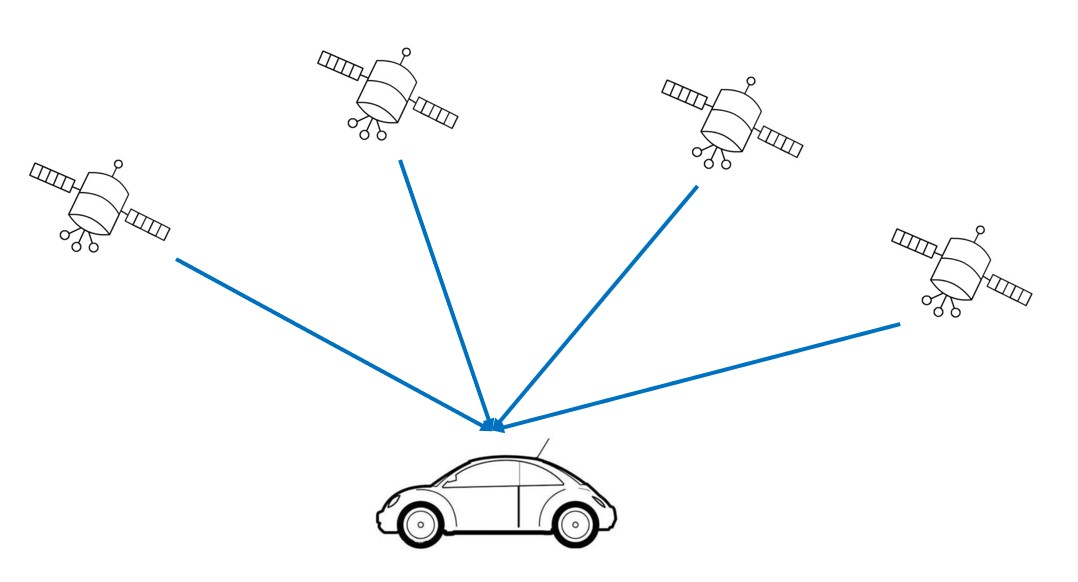
\includegraphics[scale=0.4]{./figures/gps.jpg}
	\caption{the GPS Positioning Module}
	\label{fig:gps}
\end{figure}


\subsubsection{Wi-Fi Fingerprint Positioning module}
Under normal circumstances, the RSSI values of Wi-Fi or Bluetooth in various indoor areas are different to different degrees, and the geomagnetic signals everywhere are also different due to the influence of buildings. Using these differences, select location reference points from indoors, and collect location fingerprint information on these points to build a fingerprint database, and save the mapping relationship between each reference point and fingerprint information. The position of the reference point should be determined according to the accuracy supported by the signal source, and should be distributed as evenly as possible and cover various indoor areas. There are usually two schemes for collecting fingerprint information: one is to collect the signal strength distribution RSSI of multiple base stations at the reference point as the characteristic information; the other is to obtain it through the signal attenuation model, combining the RSSI characteristic information and the corresponding coordinates into a position Fingerprint records. The online test phase compares the measured RSSI with the data in the fingerprint database to finally determine the location of the mobile terminal.

Location fingerprints can be of multiple types, and any ``location unique" (helpful to distinguish location) feature can be used as a location fingerprint. For example, the multipath structure of the communication signal at a certain location, whether the access point or base station can be detected at a certain location, the RSS (received signal strength) of the signal from the base station detected at a certain location, and when communicating at a certain location The round-trip time or delay of the signal can be used as a location fingerprint, or can be combined as a location fingerprint.

There are usually two phases for positioning using location fingerprints: offline phase and online phase. In the offline stage, in order to collect fingerprints at various locations and build a database, it is necessary to conduct tedious surveys in designated areas. The collected data is sometimes called a training set. In the online phase, the system will estimate the location of the mobile device to be located. Next we will describe these two stages in more detail. It should be noted that the position coordinates obtained in indoor positioning usually refer to coordinates in a local coordinate system in the current environment, rather than latitude and longitude.

The almost ubiquitous availability of WiFi makes it an attractive location method (without additional hardware costs). Location methods based on time and angle are not suitable for WiFi signals, making location fingerprinting the main choice for location. However, the location fingerprinting method requires very cumbersome data collection work, and may need to be updated frequently as the environment changes. In addition, due to the complexity of radio propagation, the collection of location fingerprints is not an easy problem in itself. Some measurement, analysis and simulation have shown that some empirical methods can be adopted to reduce the workload of fingerprint collection. If the requirements for positioning accuracy are not high, other methods such as sub-area positioning or organic construction of location fingerprints can be used to reduce the workload of fingerprint collection. An example of Wi-Fi fingerprint positioning is shown in Fig. \ref{fig:wifi}. As the current Wi-Fi fingerprint is [0.1,0.3,0.1]. It is close to [0.1,0.2,0.1], so the current position is nearby.

\begin{figure}[h]
	\centering
	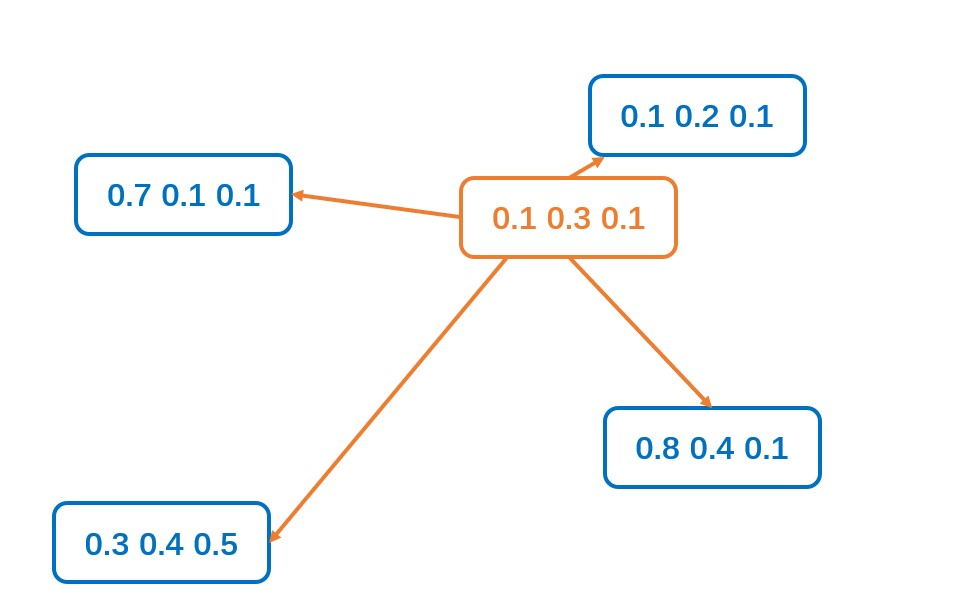
\includegraphics[scale=0.4]{./figures/wifi.jpg}
	\caption{the Wi-Fi Fingerprint Positioning Module}
	\label{fig:wifi}
\end{figure}

\subsubsection{PDR Positioning module}

Inertial navigation mainly uses the built-in sensors in the device to obtain data such as acceleration and heading angle to calculate the pedestrian step length and walking direction, and to estimate the pedestrian's walking trajectory indoors. With the rapid development of micro-electromechanical systems (MEMS), the sensitivity of inertial sensors such as accelerometers, gyroscopes, and magnetometers integrated on smartphones is getting higher and higher. Pedestrian track estimation systems (PDR) based on inertial sensors are becoming more and more popular. The more attention. Pedestrian track estimation algorithm uses the acceleration sensor to obtain the acceleration of the user while walking to determine the number of walking steps, and then multiply it by the step length to obtain the walking distance. According to the gyroscope data to obtain the user’s walking direction, it can be inferred based on the data at the previous moment The current location of the user.

Because everyone has different heights, weights, and walking styles, there is a big difference in step length when walking. Even the same person, under different conditions, can hardly maintain the same pace. In the PDR positioning system based on inertial sensors, the step size error will continue to accumulate as the user's walking time increases. Therefore, the difficulty lies in the calculation of the step length L. People are very individual creatures. Different people, different environments, and different dresses have different steps. To put it bluntly, there is no good calculation formula to simulate. Human step length, of course, this also causes errors.

In time, some papers produced the inertial system they designed with an accuracy of less than 1\%. In fact, if you look carefully, their experimental scenes are often limited to a very small range and the time span is also very short. Imagine you go out shopping. You may be in a large shopping mall for several hours. At this time, the inertial navigation system has already turned to the horizon. This is the current business scenario, and no pure inertial navigation system can be successful. The principleof PDR positioning module is shown in Fig. \ref{fig:pdr}.

\begin{figure}[h]
	\centering
	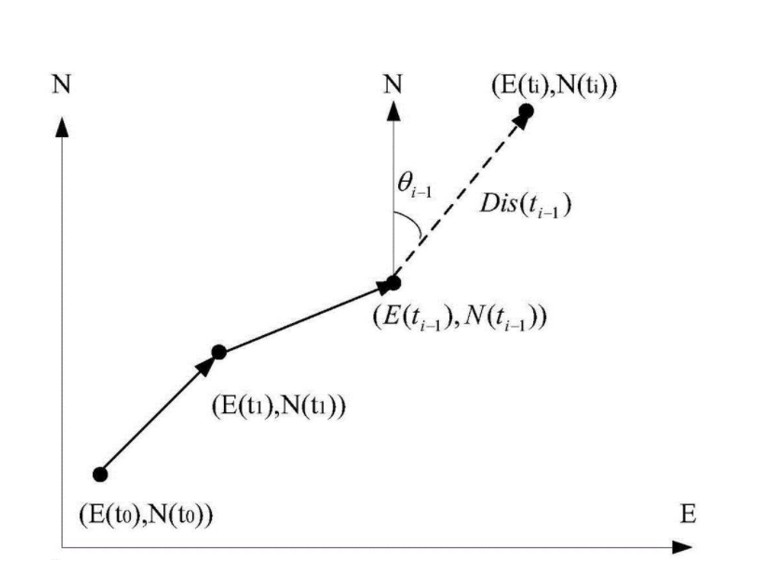
\includegraphics[scale=0.4]{./figures/pdr.jpg}
	\caption{the PDR Positioning Module}
	\label{fig:pdr}
\end{figure}

\subsection{LSTM-Based Weight Adjustment}
LSTM \cite{lstm} is a neural network with excellent RNN structure at present, which is particularly effective for processing time series data. At present, LSTM has achieved a series of excellent experimental results. \cite{lstm-1} utilizes LSTM to do trajectory prediction. \cite{lstm-attention} utilizes both LSTM and attention mechanism for urban vehicle trajectory prediction. \cite{lstm-sr} raised SS-LSTM while \cite{lstm-ss} raised SS-LSTM for pedestrian trajectory prediction. \cite{lstm-cnn} combined LSTM with CNN for Motion trajectory prediction.

The movement trajectory of the device is natural time series data, so in the SPAE model, we use the LSTM network to dynamically adjust the weights of the three positioning modules. The specific method is that in the training phase, the training data is the positioning coordinates output by the three positioning modules, and the label data is the real coordinates of the device. We hope that LSTM can learn the weight relationship of the three positioning modules in different scenarios. The overall view of our SPAE model is shown in Fig. \ref{fig:spae}.

In addition, in order to prevent abnormal deviations in LSTM, we set a threshold based on GPS signal strength. When the GPS signal is greater than the threshold, the GPS positioning module will be forced to be used first, which is reflected in the SPAE model to increase the weight of the GPS positioning module. This mechanism can effectively prevent the occurrence of position drift.

\begin{figure}[h]
	\centering
	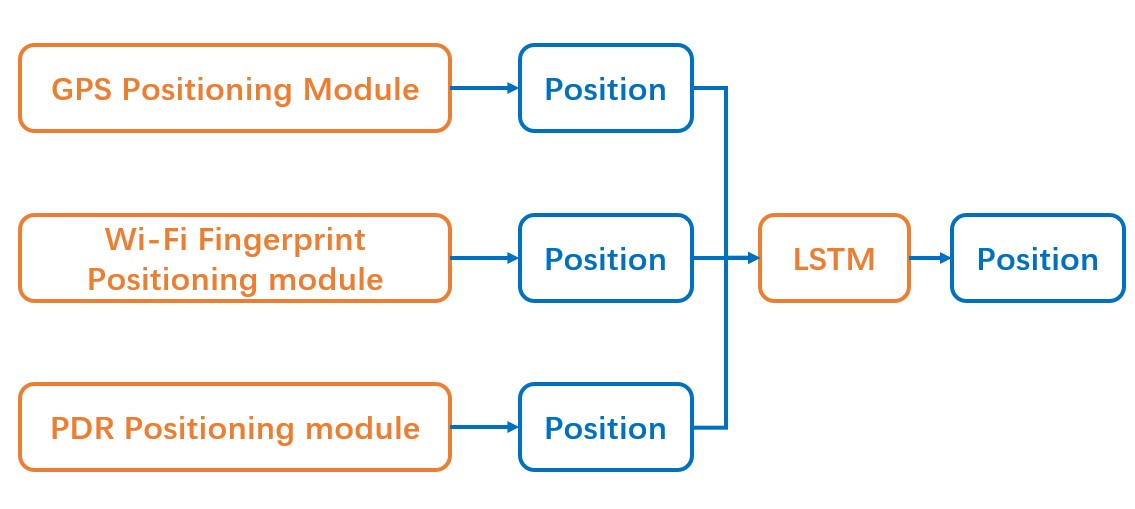
\includegraphics[scale=0.3]{./figures/spae.jpg}
	\caption{the Overview of SPAE Model}
	\label{fig:spae}
\end{figure}

\section{Experiments and Results}
In order to verify the correctness of the SPAE model and test the performance of the SPAE model, we set up three experiments. The purpose of experiment one is to verify the correctness of the SPAE model and also to verify the correctness of the program code. Experiment 2 tested the working condition of the SPAE model in a simple scenario, and experiment 3 tested the working condition of the SPAE model in a complex and complex situation.

Our experimental environment is as follows. The operating system we use is Ubuntu 20.04, the CPU model is Intel(R) Core(TM) i7-700HQ @ 2.80GHz, and the memory is 16 GB. We use anaconda for python environment and package management, and the python version used is 3.8.5. We use Python to build a simulated virtual environment for experiments. The simulation environment can simulate GPS signal conditions and Wi-Fi signal conditions in different scenarios, and can add random electromagnetic noise and random environmental disturbances.

We utilize a exponential function to measure the score of two distances. Suppose that two positions $p_1=(x_1,y_1,z_1)$ and $p_2=(x_2,y_2,z_2)$. We define a function $s(\cdot,\cdot)$ to measure the similarity between $p_1$ and $p_2$. The value of $s(\cdot,\cdot)$ should be $1.0$ if $p_1=p_2$ while be near $0.0$ if $p_1$ is far from $p_2$. We define $s(\cdot,\cdot)$ as follow:

\begin{equation}
	s(p_1,p_2)=exp\left( - A \cdot d(p_1,p_2) \right)
\end{equation}

where $d(\cdot,\cdot)$ is the 3-dimensional Euclidean distance defined as follow:

\begin{equation*}
d(p_1,p_2)=\sqrt{(x_1-x_2)^2+(y_1-y_2)^2+(z_1-z_2)^2}
\end{equation*}

\begin{figure}[h]
	\centering
	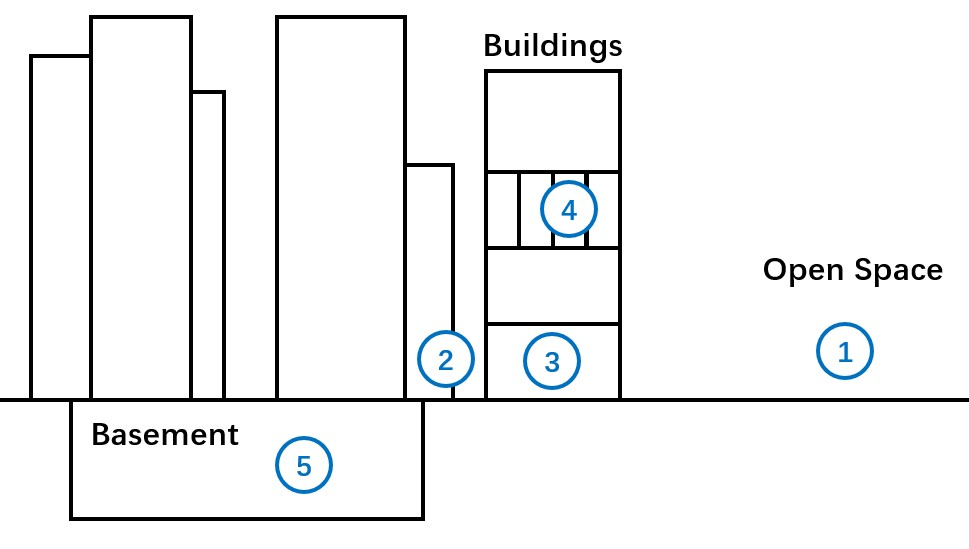
\includegraphics[scale=0.3]{./figures/scenes.jpg}
	\caption{the General View of All Five Scenes}
	\label{fig:scenes}
\end{figure}

In the first experiment, we constructed five basic virtual scenes, namely 1) an open outdoor environment; 2) an outdoor environment with high-rise buildings nearby; 3) a shopping mall indoor environment with a larger space; 4) a small space Hotel indoor environment; 5) basement environment. The environmental parameters of each scene are shown in Table \ref{tab:scenes} and the general view is shown in Fig. \ref{fig:scenes}.

\begin{table}[h]
	\centering
	\caption{the Parameters of All Five Scenes}
	\label{tab:scenes}
	\begin{tabular}{llll}
		\hline
		ID & Description     & GPS Signal & Wi-Fi Signal \\ \hline
		1  & Open Outdoor    & 10.0       & 0.0          \\
		2  & Narrow Outdoor  & 8.0        & 1.0          \\
		3  & Large Indoor    & 3.0        & 9.0          \\
		4  & Small Indoor    & 2.0        & 10.0         \\
		5  & Basement Indoor & 1.0        & 3.0          \\ \hline             
	\end{tabular}
\end{table}

We tested the positioning of the SPAE model in each scene. In different scenarios, the weight of each positioning module and the positioning performance are both shown in Table \ref{tab:exp1}. It can be seen that in different scenarios, the SPAE model can select appropriate weights to dynamically adjust the proportion of positioning modules to achieve the optimal positioning performance.

\begin{table}[h]
	\centering
	\caption{the Weight of All Three Modules}
	\label{tab:exp1}
	\begin{tabular}{lllll}
		\hline
		ID & Weight of GPS & Weight of Wi-Fi & Weight of PDR & Accuracy \\ \hline
		1  & 1.00          & 0.00            & 0.00          & 0.97     \\
		2  & 0.76          & 0.22            & 0.02          & 0.86     \\
		3  & 0.12          & 0.85            & 0.03          & 0.75     \\
		4  & 0.06          & 0.90            & 0.04          & 0.72     \\
		5  & 0.04          & 0.54            & 0.42          & 0.61     \\ \hline             
	\end{tabular}
\end{table}

In the second experiment, we moved the device in five scenes to detect the working condition of the SPAE model in a simple scene. We take the parameter $A=1$. The experimental results are shown in Fig. \ref{fig:e2}. It can be seen that when the device moves from one scene to another, the SPAE model automatically recognizes the changes in the scene and dynamically adjusts the weight of each positioning module.

\begin{figure}[h]
	\centering
	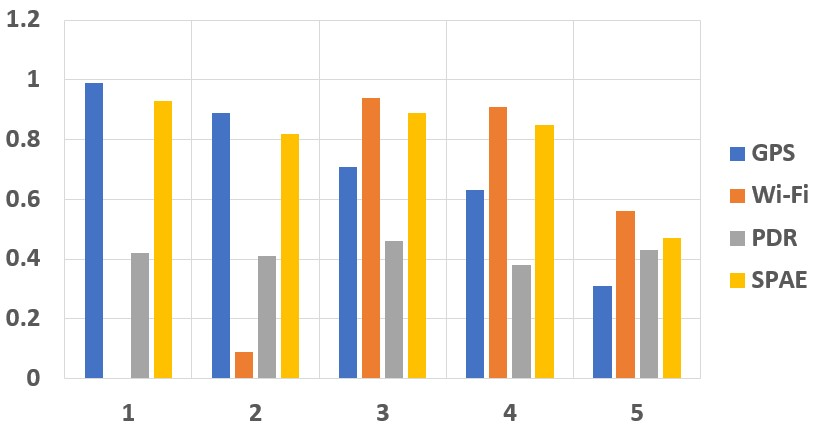
\includegraphics[scale=0.5]{./figures/e2.jpg}
	\caption{the Results of Experiment 2}
	\label{fig:e2}
\end{figure}

In the third experiment, we moved the equipment in five scenes. Unlike Experiment 2, we added random electromagnetic noise and random environmental disturbances to simulate irregular electromagnetic signals and uneven environments in the real environment. Disturb. The experimental results are shown in Fig. \ref{fig:e3}. It can be seen that our SPAE model can better adapt to this random environment, and adjust the parameters of each positioning module as much as possible to obtain relatively accurate positioning.

\begin{figure}[h]
	\centering
	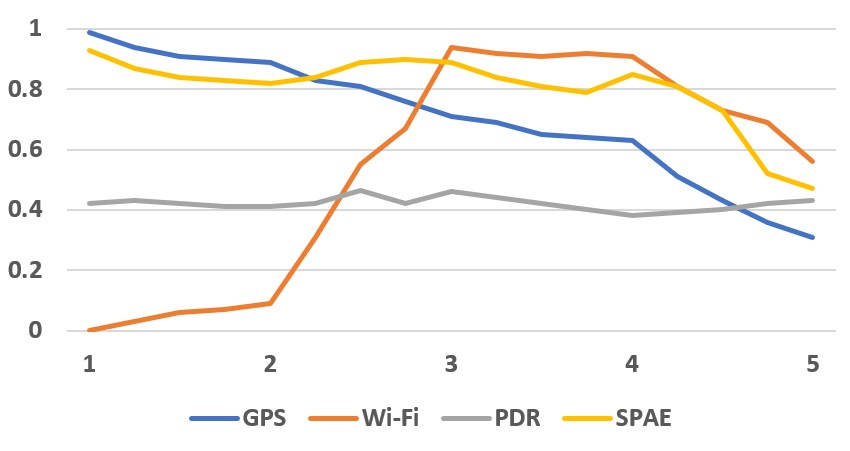
\includegraphics[scale=0.5]{./figures/e3.jpg}
	\caption{the Results of Experiment 3}
	\label{fig:e3}
\end{figure}

\section{Conclusion}
From the Internet to the Internet of Things, location has always been an indispensable information. The higher the positioning accuracy, the greater the availability of location information. From the perspective of positioning scenarios, positioning can be divided into two types: outdoor positioning and indoor positioning. The mainstream technologies for outdoor positioning include GPS positioning and LBS positioning. The mainstream technologies for indoor positioning include wireless signal intersection positioning, Wi-Fi fingerprint positioning, and PDR positioning. In recent years, the development of deep learning is in full swing. The neural network framework LSTM used to realize deep learning has long-term memory function and is favored by the majority of researchers. Many works apply LSTM to indoor positioning to improve the accuracy of positioning. The SPAE model proposed in this paper integrates three different positioning algorithm modules, and applies the LSTM network to the weight adjustment, which can realize dynamic positioning model adjustment in a complex environment.

The next research direction of this article is to expand the data set used for LSTM training, because the neural network can only obtain better performance when it is trained with a large sample. The second is to support the expansion of multiple positioning models. This article only supports three algorithms: GPS positioning, Wi-Fi fingerprint positioning, and PDR positioning. If a new positioning algorithm is added, the entire LSTM network must be retrained. How to perform model reuse of LSTM in the case of newly added positioning algorithms is a very important topic.

\bibliographystyle{./bibliography/IEEEtran}
\bibliography{./bibliography/IEEEabrv,./bibliography/references}

\end{document}
